%!TEX root = SysSpec_ClockPendulumAnalyzer.tex
\section{Systemdesign}
    Im Kapitel Systemdesign wird die Umsetzung einzelner Komponenten sowie der gesamte Kontext des CPA erklärt.
        \subsection{Kontextdiagramm}
        Der CPA Kontext wird mittels untenstehendem Diagramm dargestellt. Das Projekt umfasst ein tinyK20 als Hardware Counter, ein Raspberry Pi als Recheneinheit und ein Sensor Board auf dem ein Infrarotsensor montiert ist.\\
        Für die Benutzerinteraktion wird ein UserInterface definiert und ein Web Client erstellt. Das UserInterface ermöglicht es weitere Benutzerschnittstellen an den CPA zu hängen. Zum Beispiel eine Qt Applikation.
        \begin{figure}[H]
            \centering
            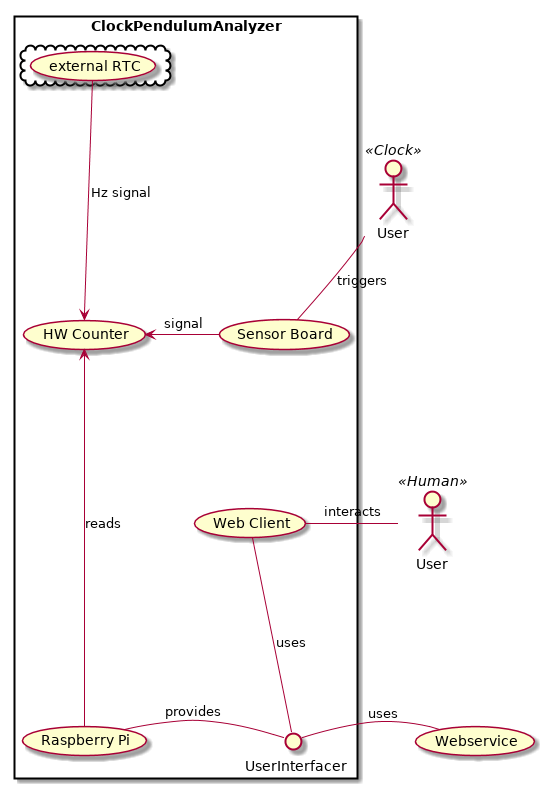
\includegraphics[width=.7\textwidth]{context.png}
            \caption{erweitertes Kontextdiagramm}
        \end{figure}

    	\subsection{Umsetzung des Clock Update}
		\subsection{Umsetzung des GPIO Zugriff}
		\subsection{Umsetzung des Hardware Counter}
        %!TEX root = SysSpec_ClockPendulumAnalyzer.tex
\subsection{Umsetzung der Datenpersistenz}
    Hier stehen Details zur Umsetzung der Datenspeicherung auf dem Raspberry Pi.
    \subsubsection{Datenspeicher}
    Da das Operationssystem des Raspberry Pi auf einer SD Karte gespeichert ist, empfiehlt es sich eine Alternative zu finden. SD Karten sind nicht für häufige Schreibzyklen ausgelegt. Für den Clock Pendulum Analyzer wird deshalb ein USB Speicher verwendet. Auf diesem wird die ganze Datenbank abgelegt.\\
    Der Datenspeicher wird beim Autostart über die \textit{/etc/fstab} Datei automatisch eingebunden.
    
    \subsubsection{SQLite als Datenbank}
    C++ bietet eine grosszügige Schnittstelle für SQLite Datenbanken. Durch SQLite braucht die Applikation auch keine umständliche Datenbankinstallation wie es bei MySQL der Fall wäre, da SQLite nur normale Dateien zum Aufbau verwendet.
    
    \subsubsection{Architektur und Beispielverwendung}
    Die Software speichert die folgenden Daten in einer einzelnen Tabelle ab.
    \paragraph{clock:}
    Der Wert in \textit{clock} hält den Namen fest der Uhr, von der die weiteren Daten stammen. Dieser wird beim Programmstart mitgeteilt.\\
    Das Feld ist vom Typ TEXT und besteht aus alphanumerischen Zeichen die der Regular Expression $$[a-zA-Z0-9]\{1,\}$$
    \paragraph{date:}\label{sec:db_date}%TODO datumsformat anpassen +zeit
    In diesem Feld steht der Zeitpunkt zu welchem der Datenwert entnommen wurde. Dazu wird die Systemzeit des RPi3 gespeichert und anschliessend so konvertiert, dass der Zeitstempel im Format \textbf{yyyyMMdd} gespeichert werden kann\\
    Das Feld ist vom Typ INTEGER und entspricht der Regular Expression
    $$[0-9]\{8\}$$
    \paragraph{absolutetime:}
    Hier steht der aktuell gemessene Zeitwert in absoluter Zeit. Der Wert bezieht sich auf die aktuell vergangenen Nanosekunden in einem Tag. Er startet bei 0:00 und läuft einen Tag.\\
    Das Feld ist vom Typ INTEGER und entspricht der Regular Expression
    $$[0-9]\{1,15\}$$
    \paragraph{heat:}
    Das Feld heat wird für den optionalen Teil Temperatureinfluss benötigt. Zum jetzigen Zeitpunkt ist dieses Feld mit 0 initialisiert.
    Das Feld ist vom Typ INTEGER und entspricht der Regular Expression
    $$[0-9]\{1,2\}$$
    \paragraph{humidity:}
    Das Feld humidity wird für den optionalen Teil Feuchtigkeitseinfluss benötigt. Zum jetzigen Zeitpunkt ist dieses Feld mit 0 initialisiert.
    Das Feld ist vom Typ INTEGER und entspricht der Regular Expression
    $$[0-9]\{1,2\}$$
    %TODO beispielverwendung einfügen
        \subsection{Umsetzung des UI}
		\subsection{Sequenzdiagramm}
			\textit{wie ein spezieller Ablauf funktioniert}
        \clearpage
		%!TEX root = SysSpec_ClockPendulumAnalyzer.tex
\subsection{Klassendiagramm}
Die Klassen der Software arbeiten nach dem folgenden Klassendiagramm. Es umfasst eine Implementierung der REST Definition und Klassen für die Datenbankanbindung an SQLite.
\begin{figure}[H]
    \centering
    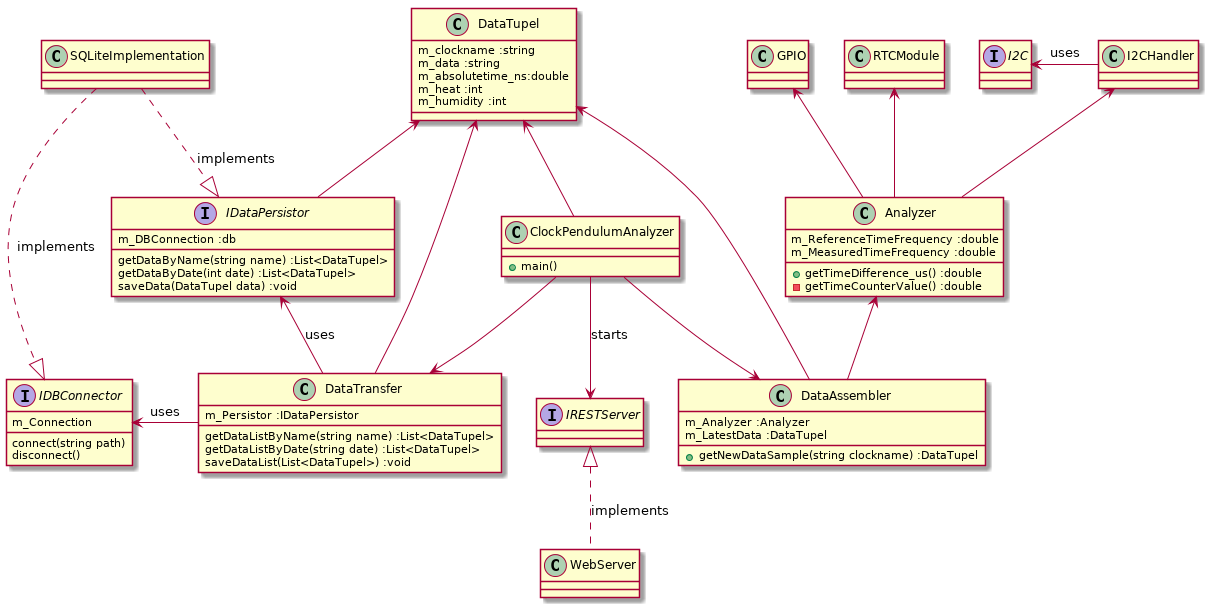
\includegraphics[width=\textwidth]{classdiagramm.png}
    \caption{Klassendiagramm der C++ Software auf dem Raspberry Pi}
\end{figure}
\subsubsection{Klassdetails}
    %TODO subject to change
	\begin{description}
        \item[ClockPendulumAnalyzer] Dies ist die Main Klasse. Sie startet alle Aufgaben.
        \item[I2CHandler] Diese Klasse öffnet und schliesst den $I^2C$-Bus und liest Daten von daran angeschlossenen Geräten.
        \item[GPIO] Eine Klasse die für das Arbeiten mit GPIO Pins auf dem Raspberry Pi zuständig ist.
        \item[Analyzer] Die Klasse ist für die Berechnung der Zeitdifferenz in Nanosekunden zuständig. Es kann auch die Differenz in Mikro- und Millisekunden ausgegeben werden.
        \item[DataAssembler] Die Klasse ist für das Zusammenfügen von Name (aus der Main Klasse) und den einzelnen Dateninputs aus dem Analyzer zuständig. Im Sequenzdiagramm ist dieser Ablauf dargestellt. 
        \item[DataTransfer] Diese Klasse ist für den Transport der DataTupel zwischen Webserver, Mainklasse und Datenbank zuständig.
        \item[DataTupel] Ein Daten Transfer Objekt (DTO) als Abstraktion der gemessenen Daten zu einem gegebenen Zeitpunkt. Beinhaltet Datum+Zeit, Name, Differenz und Werte für Feuchtigkeit und Wärme.
        \item[SQLiteImplementation] Die Implementierung der Schnittstelle \textit{IDataPersistor} und der \textit{IDBConnector} auf eine SQLite Umgebung.
    \end{description}
